
We evaluated \system{} on the three workloads motivated in \autoref{sec:intro}. We first describe our current prototype, a \system{} program for each workload, and our evaluation methodology. We then examine two experimental claims. First, \system\ can use
 its implemented physical optimizations (model selection, code synthesis, multi-data prompt marshaling, and input token reduction) to obtain physical plans that offer diverse performance trade-offs, some of which are more appealing than unoptimized naive plans. Second, the \system\ optimizer can predict plan properties quickly and accurately enough to choose a plan that fits user preferences better than unoptimized naive plans. Finally, we showcase \system{}'s ability to leverage system parallelism to minimize workload runtimes.


\subsection{Our Prototype}

We have implemented an early \system\ prototype in about 9,200 lines of Python code, which we have made available at \url{https://github.com/mitdbg/palimpzest}. It implements the operators in \autoref{fig:algebra}, and can run many programs, including the three test workloads described in \autoref{sec:intro} --- Legal Discovery, Real Estate Search, and Medical Schema Matching.

We have implemented four of the optimizations described in \autoref{sec:optimizations}: model selection, code synthesis, multi-data prompt marshaling, and input token reduction. We currently test the system using the {\tt gpt-3.5-turbo-0125}, {\tt gpt-4-0125-preview}, and {\tt gpt-4-vision-preview} OpenAI models~\cite{openaiapi} and the {\tt Mixtral-8x7B-Instruct-v0.1} model served by the Together.ai API~\cite{togetherai}. We also use the Modal online service~\cite{modalapi} for bulk non-AI function execution, such as parallel PDF processing and equation image extraction and conversion. We have tested the system with local model execution (via the Ollama~\cite{ollamawebsite} framework), but so far we have rarely found this to be an appealing option.

\system{} is implemented using the iterator model. Thus, plan execution proceeds one record at a time with each operator blocking until it receives the necessary input record(s) from its source operator(s). For clarity's sake, most of our experiments report simple single-threaded execution time, so we can better show the work saved by system optimizations.  However, many operations --- including the convert operator --- have parallel implementations that take advantage of parallelism offered by the underlying service or hardware, and we report a few parallel numbers.

\subsection{Evaluation Workloads}
We evaluated the model selection, code synthesis, and input token reduction optimizations described in \autoref{sec:optimizations} using the three workloads first discussed in ~\autoref{sec:intro}. Below, we provide details on the implementation and data used for each workload.

\begin{figure}
  \centering % breaklines
  \begin{minted}[xleftmargin=17pt,linenos,escapeinside=||,fontsize={\fontsize{8.5}{7.5}\selectfont}]{python}
import palimpzest as pz

class RealEstateListingFiles(|\textcolor{blue}{pz.Schema}|):
    """The source text and image data for a real estate listing."""
    listing = |\textcolor{blue}{pz.StringField}|(desc="The name of the listing")
    text_content = |\textcolor{blue}{pz.StringField}|(desc="The content of the listing's text description")
    image_contents = |\textcolor{blue}{pz.ListField}|(element_type=|\textcolor{blue}{pz.BytesField}|, desc="A list of the image contents")

class TextRealEstateListing(|\textcolor{blue}{RealEstateListingFiles}|):
    """Represents a real estate listing with specific fields extracted from its text."""
    address = |\textcolor{blue}{pz.StringField}|(desc="The address of the property")
    price = |\textcolor{blue}{pz.NumericField}|(desc="The listed price of the property")

class ImageRealEstateListing(|\textcolor{blue}{RealEstateListingFiles}|):
    """Represents a real estate listing with specific fields extracted from its images."""
    is_modern_and_attractive = |\textcolor{blue}{pz.BooleanField}|(desc="The home interior is modern and attractive")
    has_natural_sunlight = |\textcolor{blue}{pz.BooleanField}|(desc="The home interior has lots of natural sunlight")

def within_two_miles_of_mit(record):
    # filter based on record.address

def in_price_range(record):
    # filter based on record.price

# define logical plan
listings = |\textcolor{blue}{pz.Dataset}|(source="real-estate-eval", schema=|\textcolor{blue}{RealEstateListingFiles}|)
listings = listings.convert(|\textcolor{blue}{TextRealEstateListing}|, depends_on="text_content")
listings = listings.convert(|\textcolor{blue}{ImageRealEstateListing}|, depends_on="image_contents")
listings = listings.filter(
    "The interior is modern and attractive, and has lots of natural sunlight",
    depends_on=["is_modern_and_attractive", "has_natural_sunlight"]
)
listings = listings.filter(|\textcolor{blue}{within\_two\_miles\_of\_mit}|, depends_on="address")
listings = listings.filter(|\textcolor{blue}{in\_price\_range}|, depends_on="price")

# create and execute physical plans...
    \end{minted}
  \caption{The AI program written using \system{} for the Real Estate Search workload. 
  % In the program snippet above, we show the definition of the schemas and the creation of the logical plan. We then created a set of physical plans, executed each one, and recorded the runtime, cost, and quality of each plan.
  }
  \label{fig:real-estate-program}
\end{figure}

% Note, I avoided use of 'false positives' because this phrasing only makes sense when applied to a classifier's output. It is not appropriate for a labeled dataset

%Public interest and government lawyers frequently face the challenge of mounting a prosecution (or defense) against opponents with greater legal and financial resources. As a result, public interest lawyers are unable to spend as many hours pouring over reams of documents during legal discovery in search of evidence which would bolster their case. Such lawyers might benefit from using Machine Learning and NLP tools to automate their searches, but many existing tools require manual data labeling and are difficult for legal domain experts to use \cite{}.

  
% \begin{figure}
%   \centering % breaklines
%   \begin{minted}[xleftmargin=17pt,linenos,escapeinside=||,fontsize={\fontsize{8.5}{7.5}\selectfont}]{python}
% import palimpzest as pz

% class Email(|\textcolor{blue}{pz.TextFile}|):
% """Represents an email, which can subclass a text file"""
%   sender = |\textcolor{blue}{pz.Field}|(desc="The email address of the sender", required=True)
%   subject = |\textcolor{blue}{pz.Field}|(desc="The subject of the email", required=True)

% # define logical plan
% emails = |\textcolor{blue}{pz.Dataset}|(source="enron-eval", schema=|\textcolor{blue}{Email}|)
% emails = emails.filter("The email is not quoting from a news article or an article ...")
% emails = emails.filter("The email refers to a fraudulent scheme (i.e., \"Raptor\", ...")

% # create and execute physical plans...
%     \end{minted}
%   \caption{The AI program written using \system{} for the Legal Discovery workload.} % It begins with the definition of the Email schema followed by the creation of program code, from which a logical plan is derived. Subsequently, a set of equivalent logical plans and their corresponding physical plans were created, executed, and evaluated based on runtime, cost, and quality metrics.
%   \label{fig:enron-email-program}
% \end{figure}

{\bf Legal Discovery.} We implemented this task using the source code shown in \autoref{fig:enron-email-program}.  The program loads the raw text files and stores their {\tt filename} and {\tt contents} in a {\tt pz.TextFile}. On line 9, the program converts the input data to the {\tt Email} schema, computing the {\tt sender} and {\tt subject} fields. Lines 10 and 11 filter the email by content. 

We created a test dataset of 1000 emails drawn from the Enron email collection~\cite{enron}. This dataset was curated and labeled by hand to contain 50 examples that discuss the management of fraudulent investment vehicles, with another 30 that contain fraud-related text but are not fraudulent in nature. The remainder were randomly chosen.  We registered this set of 1000 emails using the identifier ``enron-eval". The goal of the program is to recover only those emails that indicate genuine fraudulent activity.  For all the experiments on this workload, we evaluated the F1-score of the program's output using the manual labels described above. (Of course, during optimization and plan selection, \system\ did not have access to these labels and had to estimate the plans' quality in an unsupervised fashion.)


{\bf Real Estate Search.}  Our \system{} program for this workload is shown in \autoref{fig:real-estate-program}. It has the same rough form as the Legal Discovery task above, with a few key differences.  First, because the real estate listings are multimodal, they currently do not fit into a single core library schema such as {\tt pz.TextFile}. Thus, we first define a few utility schemas. {\tt RealEstateListingFiles} stores the raw image and text data for each listing; the data loading is performed by a simple user-defined datasource that we have omitted for brevity. We also define {\tt TextRealEstateListing} and {\tt ImageRealEstateListing} for the text and image attributes that we wish to compute~\footnote{At the moment, writing two schemas is necessary because schemas and convert operations have a one-to-one relationship in our system, but in the future we plan to support splitting a single schema conversion across multiple convert operations.}.  Second, on lines 33 and 34 the user provides user-defined functions for selection, instead of text strings.  Finally, several operations on lines 27-34 use the {\tt depends\_on} parameter (which was described in \autoref{sec:logical_opt}), in this case, allowing the system to skip image processing entirely.

We manually scraped 100 real estate listings from Boston and Cambridge, MA to obtain their natural language text descriptions and the first three deduplicated images from each listing.  We registered this dataset using the identifier ``real-estate-eval".  For each listing we manually labeled whether it satisfied the location, price, and "attractive and modern" and "natural sunlight" criteria, allowing us to compute an F1-score for any program output. Overall, 23 of the 100 data items satisfied all criteria.


{\bf Medical Schema Matching.} The \system\ program for this task is shown in \autoref{fig:medical-schema-matching-program}. This program aims at reproducing the output of the data harmonization pipeline performed by the authors of~\cite{li2023proteogenomic}.
The authors provide a single table produced as the result of collecting data from 11 different experimental studies. In this original study, all tables from the various studies were manually combined to create a comprehensive view of patient information related to tumor cases. This is a complex and time-consuming task, even for domain experts. According to the author contribution section, 66 out of 79 paper authors focused on the data curation task. However, with \system, we can implement the pipeline in approximately 30 lines of code. Lines 3-21 of the program reflect a detailed description of the target output schema, as described in the paper. This program is similar to the programs for Legal Discovery and Real Estate Search, but its unique feature is the use of the {\tt cardinality} parameter, which allows \system\ to yield multiple output objects from a single input object, i.e., multiple tables from a single spreadsheet, and multiple case data from the tables.

We curated a dataset of 11 spreadsheet files --- containing a total of 49 tables --- from the supplemental data provided in the original works~\cite{Cao_2021, Clark_2019, Dou_2020, Huang_2021, Li_2023, Gillette_2020, Krug_2020, McDermott_2020, Satpathy_2021, Vasaikar_2019,Wang_2021}. 
In Figure~\ref{fig:medical-schema-matching-program}, we refer to this dataset as ``medical-eval''. The first goal of the program is to filter, out of the 49 input tables, only those which contain information about patient case data. Once these tables are identified, the program aims at mapping each column in the source tables to a target column in a set of 15 attributes. This task is very challenging: not all target attributes can be found in all source tables, and neither there is guarantee that matching columns in the source tables have the same representation as the target columns.

% In order to report quality of the program output, we manually labeled the column from each source that contained the correct values for each of the extracted target table attributes. If no column from a source table contained any of the values for a given target attribute, then we marked attribute as missing. 
For this workload, we measure accuracy using manually annotated ground truth data matching the columns from the source tables to those of the harmonized table provided by the authors of~\cite{li2023proteogenomic}.
We report the micro-average of the F1-score across all target attributes and paper studies. 

% In order to report quality of the program output, we manually labeled the column from each source table that contained the correct values for each target table column. We measured the performance of correctly predicted matches using the micro-average of the F1-score across all target attributes and paper studies. 

%\mike{can we say something about how closely this emulates the original paper?} \matt{Matt: If we did want to, Gerardo would need to be the one to explain that b/c I have not read the original paper. I do know that we automated some steps (e.g., extracting/downloading the spreadsheets from URLs). Personally, I think many readers will not get into these weeds.}
%\mike{The original writeup mentioned how we approximate the F1 by sampling; is that still true?} \matt{Matt: I think what Gerardo meant was that we only look at the first 5 rows per-column? I don't think we are subsampling columns when computing the eval? (Unless Gerardo did this in pre-processing)}
%\st{Overall, these 11 files contained 49 individual sheets, from which a single table needs to be extracted with 15 attributes. Not all attributes in the output table can be found in the source data tables. In order to report quality of the program output, we manually labeled the column from each source that contained the correct values for each of the extracted target table attributes. If no column from a source table contained any of the values for a given target attribute, then we marked attribute as missing. We measured the performance of correctly predicted matches using the micro-average of the F1-score across all target attributes and paper studies. Due to the large number of manual labels required, we approximated the F1 answer by labeling the first 5 rows from each source table.}


\subsection{Optimizations Produce Plans with Diverse Performance Trade-offs}
\label{sec:opt-and-tradeoffs}

\begin{figure}[h]
    \centering
    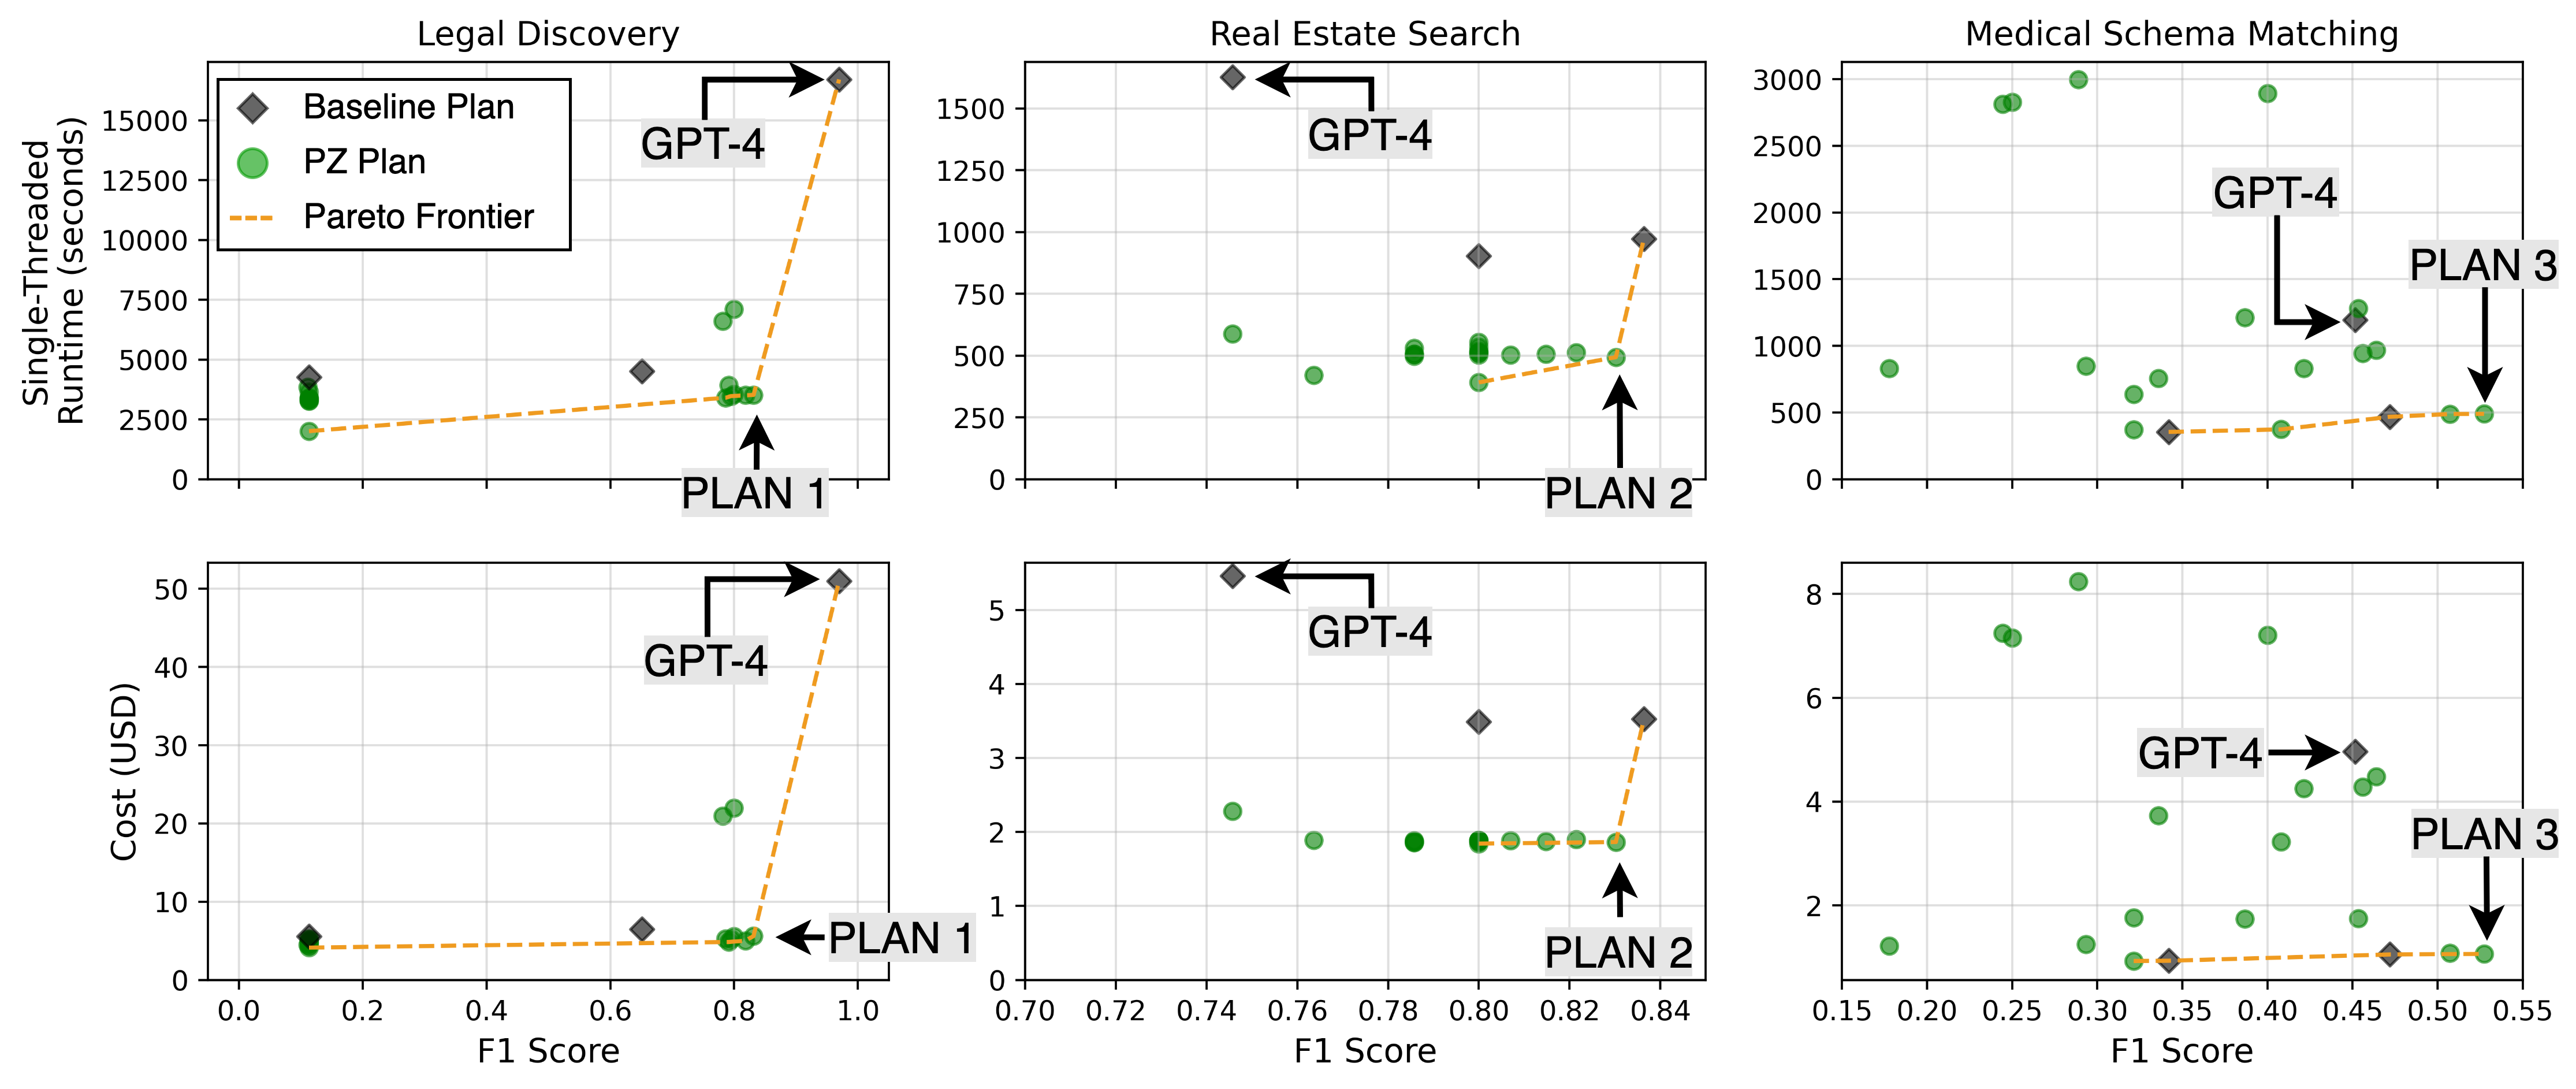
\includegraphics[width=0.95\textwidth]{imgs/all-plans.png}
    \caption{Performance of different plans on each workload (plans towards the bottom-right of each subplot are better). Naive plans are depicted with black diamonds and plans which \system{} creates with its physical and logical optimizations are shown with green circles. Across all workloads, \system{} produces plans on the Pareto frontiers of runtime vs. quality and cost vs. quality.}
    \label{fig:all-plans}
\end{figure}

Our first experimental claim is that \system\ can use its three optimization strategies to create a set of physical plans that offer appealing trade-offs regardless of the user policy.  To evaluate this claim, for each workload we ran \system{} up to (but not including) the final step in Algorithm~\ref{algo:optimization}. We then took the set of frontier plans, three baseline plans, and the top-$k$ plans from the {\it reducedCandidates} that were closest to the approximated Pareto frontier, such that we ultimately executed 20 plans in total. Our three baselines were the naive physical plans for each workload which used only GPT-4, GPT-3.5, or Mixtral-8x7B, respectively. The optimizer's compilation process took 2.6s, 13.1s, and 2.7s for Legal Discovery, Real Estate Search, and Medical Schema Matching, respectively.

Figure~\ref{fig:all-plans} shows the observed runtime, cost, and quality that came from executing all the aforementioned plans. Some plans exhibit similar performance, which makes them overlap in the figure, thereby presenting fewer than 20 distinct visual data points. Plans closer to the bottom-right of each subplot are better. Note that data points reflect observed values, not the system's estimated ones. During sample-based statistics collection, we used 5\% of the workload's total input size to run our sentinel plans, which gathered data to help estimate the cost of all plans. The one exception to this was the Medical Schema Matching workload, where we used 1 out of 11 inputs to gather sample data.
% \system{} used the naive plans for each workload as its sentinels.  % We have highlighted the sentinel plans, the plans chosen by \system\ when trying to optimize for user policies {\bf Policy-A} and {\bf Policy-B}, and the best available plans under those two policies.


We found that \system{} is able to create useful plans at a number of different points in the trade-off space. On the Legal Discovery workload, \system{} was able to suggest physical plans (e.g. PLAN 1) that dominated the GPT-3.5 and Mixtral baselines, with an F1-score that is 7.3x and 1.3x better (respectively) at lower runtime and cost. Compared to the GPT-4 baseline, \system{} produced a cluster of plans near PLAN 1 that are $\sim$4.7x faster and $\sim$9.1x cheaper, while still achieving up to 85.7\% of the GPT-4 plan's F1-score.

The physical plan for PLAN 1 is shown in the Appendix. It achieved lower runtime and cost compared to the GPT-4 baseline plan by judiciously applying GPT-3.5 and Mixtral to the convert and filter operation(s). In particular, the plan did {\it not} use GPT-3.5 on the filter for fraudulent entities and did {\it not} use Mixtral on the filter for quotes from news articles. The models' poor performance on those filters, respectively, accounts for the worse performance of the baseline plans using only GPT-3.5 and only Mixtral. It is also worth noting that plans which used code synthesis for the convert operation provided speed-ups on that operation (with similar quality) relative to identical plans which used LLMs.  

On the Real Estate Search workload, where \system{} once again generated physical plans which offer desirable trade-offs relative to baseline plans. \system{} was able to produce physical plans (e.g. PLAN 2) that obtained 3.3x lower runtime, 2.9x lower cost, and up to 1.1x better F1-score than the GPT-4 baseline. These performance improvements are especially impressive considering the majority of the cost and runtime on this workload are dominated by calls to the vision model --- which cannot be optimized away using the methods in our current prototype. (In the future, we will explore options for visual processing optimizations.)

The physical plan for PLAN 2 is shown in the Appendix. It achieved improved performance relative to the GPT-4 baseline through the combination of two optimizations. First, the plan re-ordered the execution of the convert and filter operations such that the text-based operators were executed prior to image-based operators. This provided significant runtime and cost savings by avoiding calls to the GPT-4 vision model altogether. Second, the plan used input token reduction to trim the real-estate listing text by 50\%. This technique was particularly effective as the home address and listing price regularly appears at the top of the text for the listing.

Finally, on Medical Schema Matching --- our most challenging workload --- \system{} was able to produce plans (e.g. PLAN 3) which have $\sim2.4$x lower runtime, $\sim4.6$x lower cost, and up to 1.2x better F1-score than the GPT-4 baseline. This workload is especially challenging for \system{} because the code synthesis and token reduction optimizations are not very effective, but the system still identified plans that completely dominate the performance of a GPT-4 baseline.

The physical plan for PLAN 3 is shown in the Appendix. The plan used Mixtral for the filter and convert operations with a small amount token reduction (10\% of the input text trimmed). The use of Mixtral instead of GPT-4 provided significant speedups, and also provided better quality on this workload.  

We have shown that \system{} can generate plans like PLAN 1, 2, and 3 (plan details are shown in the Appendix), which provide users with compelling performance trade-offs. However, this does not automatically confirm that \system's optimizer will choose these plans during runtime. In the following section, we demonstrate that for a variety of policies, \system's cost optimizer does indeed identify and select such plans.

% \st{We note that the system is able to hypothesize useful plans at a number of different points in the tradeoff space. Further, the {\bf Policy-A} plan chosen by \system\ is within X\% of the runtime and within Y\% of the cost of the best available plan.  For {\bf Policy-B}, the plan chosen by \system\  is within X\% of the runtime and within Y\% of the cost of the best available plan.}

% \st{We see similarly good results in the Real Estate Search workload in Figure~\ref{fig:allPlansForRealEstateSearch}, where the chosen {\bf Policy-A} plan is within X\% of the runtime and within Y\% of the cost of the best available plan.  The chosen {\bf Policy-B} plan is within X\% of the runtime and within Y\% of the cost of the best available plan.}

% \st{Figure~\ref{fig:allPlansForMedicalSchemaMatching} shows results for the Medical Schema Matching workload, which is much more challenging in general.  It is not clear how the token reduction or code synthesis optimizations could be applied effectively in this case.  Nonetheless, \system\ is able to find some appealing plans.}  % Further, the chosen plans are close to the best available.

\subsection{Cost Optimizer Selects Plans with Significant Performance Improvements}
\label{sec:overallperformance}
\begin{figure}[h!]
    \centering
    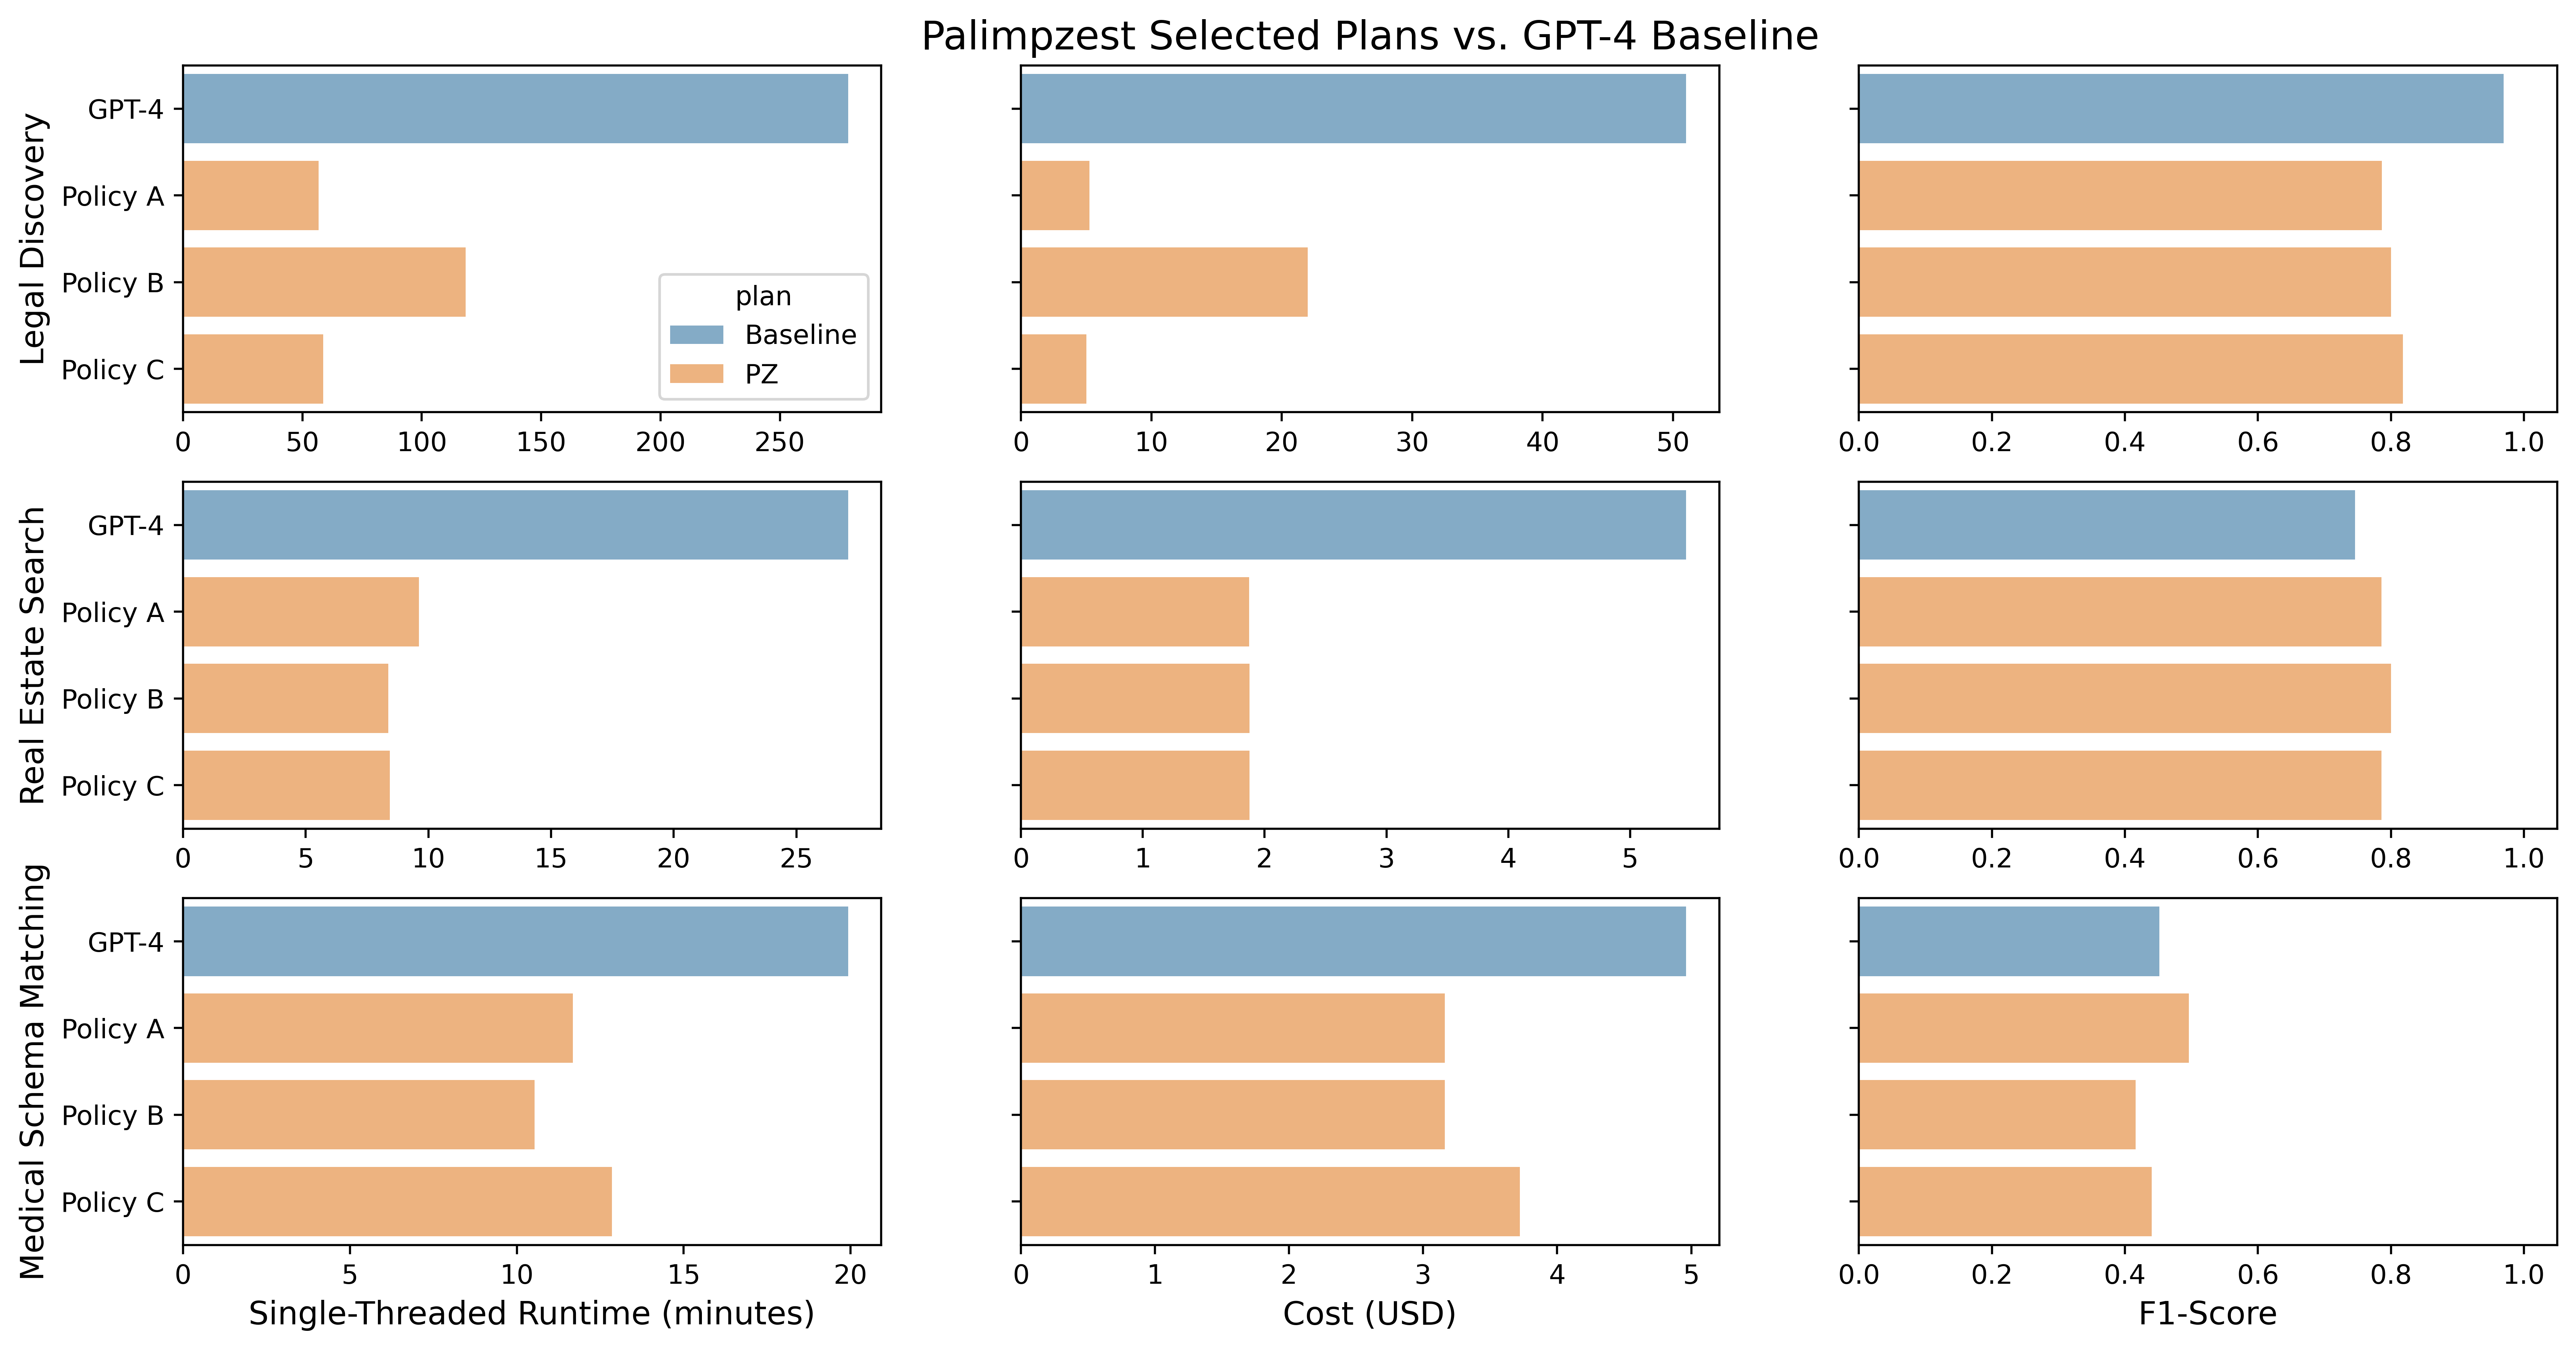
\includegraphics[width=0.95\textwidth]{imgs/reopt.png}
    \caption{Comparing the performance of plan(s) selected by \system{} to the baseline GPT-4 plan for three different policies on each workload. {\bf Policy A} maximized F1-score at cost $<$ \$20, \$3, and \$2 for each workload (top-to-bottom); {\bf Policy B} maximized F1-score at runtime $<$ 167m, 10m, and 16.7m for each workload (top-to-bottom); and {\bf Policy C} minimized cost at F1-score $>$ 0.8, 0.8, and 0.4 for each workload (top-to-bottom). \system{} consistently finds plans which provide similar F1-scores and lower costs and runtimes than the GPT-4 baseline.}
    \label{fig:reopt}
\end{figure}

Our second experimental claim is that \system\ can identify plans that have better end-to-end runtime, cost, and quality than a naive plan that uses the same state-of-the-art language model for each operation. To evaluate this claim, we ran the system as described in Algorithm~\ref{algo:optimization} --- this time including the final step which chooses the best plan for a given policy. We ran three policies for each workload. {\bf Policy A} was to maximize quality at cost $<$ \$20.0, \$3.0, and \$2.0 for Legal Discovery, Real Estate Search, and Medical Schema Matching, respectively. {\bf Policy B} was to maximize quality at runtime $<$ 10,000s, 600s, and 1000s (for the same order of workloads). Finally, {\bf Policy C} was to minimize cost at an F1-score $>$ 0.8, 0.8, and 0.4 (for the same order of workloads). These fixed cost, quality, and runtime thresholds were set to be challenging, yet physically attainable based on our results in \autoref{sec:opt-and-tradeoffs}. (The full set of thresholds can be found in \autoref{tab:policy-results}.)

\autoref{fig:reopt} presents our results across three performance metrics, with each metric displayed in a separate column. The results are organized by workload, with each workload represented in a row of subplots. Within each subplot, results are further divided by the physical plan selected by the optimizer, with each plan occupying a separate row. We compared the plans chosen by \system{} to a baseline plan, which employs GPT-4 for all conversion and filtering operations.

Overall, we found that \system{} identifies plans in the space of physical candidates which (1) offer significant performance improvements over the GPT-4 baseline, (2) generally satisfy policy constraints (7 out of 9 satisfied), and (3) have speedups and cost savings which outweigh the overhead of collecting sample data. For example, on the Legal Discovery workload (first row in \autoref{fig:reopt}), the plan selected by \system{} for {\bf Policy A} achieved a runtime and financial cost that are 80.0\% and 89.7\% lower than the GPT-4 baseline, respectively, at an F1-score within 81.1\% of the baseline. The system achieved similar results for {\bf Policy C}, with slightly better quality (within 84.3\% of the baseline).

% For the Real Estate Search workload, {\bf Policy X} is able to obtain a runtime that is X\% lower, a financial cost that is Y\% lower, and a quality that is equal to the GPT-4 plan.  For {\bf Policy Y}, the best plan yields runtime that is X1\% lower, cost that is Y1\%, and equal quality.

For the Real Estate Search workload (second row in \autoref{fig:reopt}), the plans chosen by \system{} achieved (on average) 67.5\% lower runtime, 65.7\% lower cost, and 6\% better F1-score than the baseline GPT-4 plan. Finally, on the Medical Schema Matching workload (third row in \autoref{fig:reopt}), \system{} was able to identify plans that provide up to 47.2\% and 36.3\% lower runtime and cost, respectively, at comparable F1-scores to the GPT-4 baseline.

\begin{table}
    \centering
    \caption{\system{} satisfied the policy constraint on 7 out of 9 plans it executed in \autoref{sec:overallperformance}. Constraint thresholds were chosen to be challenging, but realistic based on our results in \autoref{sec:opt-and-tradeoffs}.}
    \renewcommand{\arraystretch}{1.3}
    \centering
    \begin{tabular}{|l|l|l|c|}
    \hline
    {\bf Policy Name} &{\bf Policy Detail} & {\bf Workload } & {\bf Actual v. Constraint} \\
    \hline
    Policy A & Max F1 @ Cost $<\$20$ & Legal Discovery & {\bf \$5.27$<$\$20} \\
    \hline
    Policy A & Max F1 @ Cost $<\$3$ & Real Estate Search & {\bf \$1.87$<$\$3} \\
    \hline
    Policy A & Max F1 @ Cost $<\$2$ & Medical Schema Matching & \$3.16$\nless$\$2 \\
    \hline
    Policy B & Max F1 @ Runtime $<$ 10000s & Legal Discovery & {\bf 7102s$<$10000s} \\
    \hline
    Policy B & Max F1 @ Runtime $<$ 600s & Real Estate Search & {\bf 502s$<$600s} \\
    \hline
    Policy B & Max F1 @ Runtime $<$ 1000s & Medical Schema Matching & {\bf 632s$<$1000s} \\
    \hline
    Policy C & Min Cost @ F1 $>$ 0.80 & Legal Discovery & {\bf 0.82$>$0.80} \\
    \hline
    Policy C & Min Cost @ F1 $>$ 0.80 & Real Estate Search & 0.79$\ngtr$0.80 \\
    \hline
    Policy C & Min Cost @ F1 $>$ 0.40 & Medical Schema Matching & {\bf 0.44$>$0.40} \\
    \hline
    \end{tabular}
    \label{tab:policy-results}
\end{table}

% For the Medical Schema Matching workload, {\bf Policy X} is able to obtain a runtime that is X\% lower, a financial cost that is Y\% lower, and a quality that is equal to the GPT-4 plan.  For {\bf Policy Y}, the best plan yields runtime that is X1\% lower, cost that is Y1\%, and equal quality.

% It is gratifying to find improvements across many different tasks and policy goals. But how effectively is \system\ able to hypothesize good plans in the first place, and how effectively can \system\ identify them?

\subsection{Minimizing Runtime with Parallel Operators}

\begin{table*}[h!]
    \caption{Runtime speedup from executing \system{} plans with parallel convert and filter operators. We compare these to the single-threaded GPT-4 baselines for each workload. All \system{} plans were selected by the system under {\bf Policy A}.}
    \begin{subfigure}{\textwidth}
        \caption{Legal Discovery}
        \vspace{-4pt}
        \renewcommand{\arraystretch}{1.3}
        \centering
        \begin{tabular}{|c|c|c|c|}
        \hline
        {\bf Plan } & {\bf Runtime (s)} & {\bf Cost (\$)} & {\bf F1}\\
        \hline
        Single-Threaded Baseline (GPT-4) & 16,712 & 51.0 & 0.97 \\
        \hline
        Palimpzest & 185 (1.1\%) & 5.60 (11.0\%) & 0.81 (83.5\%) \\
        \hline
        \end{tabular}
        \label{tab:speedup-legal-discovery}
    \end{subfigure}
    %%%%%%%%%%%%%%%%%%%%%%%%%%%%%%%%%%%%%%%%%%
    \begin{subfigure}{\textwidth}
        \caption{Real Estate Search}
        \vspace{-4pt}
        \renewcommand{\arraystretch}{1.3}
        \centering
        \begin{tabular}{|c|c|c|c|}
        \hline
        {\bf Plan } & {\bf Runtime (s)} & {\bf Cost (\$)} & {\bf F1}\\
        \hline
        Single-Threaded Baseline (GPT-4) & 1,626 & 5.46 & 0.75 \\
        \hline
        Palimpzest & 80.9 (5.0\%) & 1.86 (34.1\%) & 0.80 (107\%) \\
        \hline
        \end{tabular}
        \label{tab:speedup-real-estate}
    \end{subfigure}
    %%%%%%%%%%%%%%%%%%%%%%%%%%%%%%%%%%%%%%%%%%
    \begin{subfigure}{\textwidth}
        \caption{Medical Schema Matching}
        \vspace{-4pt}
        \renewcommand{\arraystretch}{1.3}
        \centering
        \begin{tabular}{|c|c|c|c|}
        \hline
        {\bf Plan } & {\bf Runtime (s)} & {\bf Cost (\$)} & {\bf F1}\\
        \hline
        Single-Threaded Baseline (GPT-4) & 1,195 & 4.96 & 0.45 \\
        \hline
        Palimpzest & 215 (18.0\%) & 3.36 (67.7\%) & 0.46 (102\%) \\
        \hline
        \end{tabular}
        \label{table:speedup-medical}
    \end{subfigure}
    \label{tab:speedup}
\end{table*}

%\mjf{For later, it would be good to have details on how much of the 3 optimization helped in each case}

%\mjf{Should also compare to a naive parallelized GPT 4 approach}


For our final evaluation, we ran \system{} with parallel implementations of the convert and filter operations to demonstrate the system's ability to achieve large runtime speedups --- with competitive costs and F1-scores --- relative to a single-threaded baseline plan. For each convert and filter operator we used 32 workers to execute operations in parallel. We did not pipeline operations, i.e. every record needed to be processed in a given convert or filter operation before the next operation in the plan could commence (but this is an optimization we could implement in the future). For each workload we ran \system{} and asked the optimizer to select the optimal plan according to {\bf Policy A}.

The results of our evaluation are shown in \autoref{tab:speedup}. We can see that on Legal Discovery, \system{} achieved a {\bf 90.3x speedup at 9.1x lower cost while obtaining an F1-score within 83.5\% of the GPT-4 baseline}. On Real Estate Search and Medical Schema matching, the optimized plan dominated the GPT-4 baseline on all metrics. {\bf These plans achieve better F1-scores than their baselines, and do so with speedups of 20.0x and 5.6x as well as cost savings of 2.9x and 1.5x, respectively.}

We do not use any exotic algorithms, and of course it is straightforward to run model prompts in parallel.  \system's abstractions simply allow the system to obtain these speedups with no additional work by the user.

%%%%%%%%%%%%%%%%%%%%%%%%%%%%%%%%%%%%%%%%%%%%%%%%%%%%%%%%%%%%%%%%%%%%%%%%%
%%%%%%%%%%%%%%%%%% ORIGINAL EXPERIMENTAL RESULTS %%%%%%%%%%%%%%%%%%%%%%%%
%%%%%%%%%%%%%%%%%%%%%%%%%%%%%%%%%%%%%%%%%%%%%%%%%%%%%%%%%%%%%%%%%%%%%%%%%

% \subsection{Original Experimental Results}

% For each optimization and workload, \system{} generated a set of candidate physical plans which were on the Pareto frontier of its initial cost, quality, and runtime estimates. (This did not guarantee that these plans would form a Pareto frontier in reality, \matt{but as we demonstrate in ~\autoref{sec:opt-and-tradeoffs} this set of plans ultimately provided diverse performance trade-offs}.) We then executed each plan on the estimated Pareto frontier and measured its true runtime and cost. We also computed an F1-score for each plan by comparing its output to a manually labelled groundtruth.


% In this section we demonstrate that \system{}'s optimizer can generate a wide range of plans with useful \matt{runtime, cost, and quality} trade-offs. \matt{Under normal operation, the system hypothesizes a large number of plans for a particular program and picks the best one according to its plan estimates and the stated user preference(s). However,} for the experiments in this section we formulated and ran {\em all} plans for a particular program and optimization scheme. \matt{For each optimization, we generated a set of plans by considering all combinations of the logical optimizations (i.e. filter and convert reordering) and the specified physical optimization.} We then executed each plan and measured the runtime, cost in US dollars (computed by {multiplying the token usage by} the models' posted pricing rates), and F1-score. 

% \matt{We emphasize that the plans \system{} suggests for each experiment are based on the Pareto frontier of its initial plan estimates --- which may not line up with their true costs, runtimes, and quality.} Many of these plans offer unappealing trade-offs and no rational user would choose them. Furthermore, in this section we do not examine \system's ability to predict which plan will be best (\matt{that is left for} \autoref{sec:reoptimization}). The only goal here is to show that the system generates more appealing plans than naive implementations.
 
% \vspace{0.1cm}
% \noindent {\bf Model Selection}
% \label{sec:model-selection}
% %%%%% MODEL SELECTION %%%%%
% \begin{figure*}[t!]
%     \includegraphics[width=\textwidth]{imgs/model_selection/modelsel-bw-msm.png}
%     \caption{Performance of different \system{} plans using the {\bf model selection} optimization on each workload. Naive implementations which use a single model for all operations are highlighted with tags. Plans on 2-dimensional Pareto frontiers are circled. \system{} is able to produce a diverse set of plans in the space of runtime, cost, and quality, many of which are strictly better than their naive counterparts.}
%     \label{fig:model-sel-all-results}
% \end{figure*}

% The first optimization we evaluated was model selection, which allows \system{} to consider using a different foundation model at each convert and filter operator in a given plan. \st{The intuition behind this optimization is quite straightforward: many convert and filter operations don't require the most expensive model to achieve high-quality outputs. For example, in the Legal Discovery workload, even small and inexpensive models such as Gemini can extract the email's subject and sender with near-perfect accuracy.}

% For this evaluation, we \st{had \system{}'s optimizer consider all logical optimizations (i.e. filter and convert re-orderings) as well as every permutation of model choice(s) at all convert and filter operations. We} limited \system{} to choosing models from the list of GPT-4, GPT-3.5, Mixtral 8x7B, and Gemini Pro 1.0. After enumerating all possible plans, we estimated the runtime, cost, and quality of each plan and executed the subset of plans which formed the Pareto frontier of our estimates. The results of executing each plan are shown in \autoref{fig:model-sel-all-results}.

% Our results demonstrate that plans which mix-and-match models often achieve strictly better performance than plans which do not. On the Legal Discovery workload, one Pareto optimal plan uses GPT-4 and GPT-3.5, while the other uses a combination of GPT-4, GPT-3.5, and Gemini. The latter of these two plans achieves the same F1-score as the GPT-4 plan on this dataset, but does so at 9.9x lower cost and 1.7x lower runtime. \matt{The best performing plans typically replace the sender and subject extraction with a cheap model (e.g. Gemini) but keep GPT-4 for the difficult semantic task (determining whether an email quotes from an article or not).}

% On the Real Estate Search workload, all Pareto optimal plans use multiple models. Furthermore, all of these plans perform conversion and filtering on the text attributes before performing any data processing on the listing images --- which showcases the utility of \system{}'s logical optimizations. \matt{Note that for this workload we used the GPT-4 vision model on all plans to perform the convert operation on the images, as it was far superior to the alternative Gemini vision model we considered. With the exception of the vision model, the naive implementations use a single model for the rest of the filter and convert operations.}

% Finally, on the Medical Schema Matching workload \matt{we observe that the highest F1-score is achieved by a mixed-model plan --- but the GEMINI plan achieves within 97\% of that score at technically zero cost as we used the free version of the model}. Nevertheless, \system{}'s mixed-model plans still provide the user with potentially desirable trade-offs. \matt{For example, the Pareto optimal plan using a mixture of Mixtral 8x7B and GPT-3.5 achieves within 94\% of the GEMINI plan's F1-score at 1.8x lower runtime.}


% %%%%% CODE SYNTHESIS %%%%%
% \begin{figure*}[t!]
%     \includegraphics[width=\textwidth]{imgs/code_generation/codesynth-bw-msm.png}
%     \caption{Performance of different \system{} plans using the {\bf code synthesis} optimization on each workload. Naive implementations which do not use code synthesis are highlighted with tags. Plans on 2-dimensional Pareto frontiers are circled. On the Legal Discovery and Real Estate Search workloads, \system{} is able to produce plans with code synthesis that offer different (and in some cases strictly better) performance trade-offs as compared to naive implementations.}
%     \label{fig:codegen-all-results}
% \end{figure*}


% \vspace{0.1cm}
% \noindent {\bf Code Synthesis}

% For this evaluation, we once again had \system{}'s optimizer consider all logical optimizations and allowed it to set each convert operator's execution strategy to \matt{either use an LLM or synthesized code}. To isolate the benefits of the code synthesis optimization (as opposed to e.g. model selection), we only considered plans which used a single model (one of GPT-4, GPT-3.5, Mixtral 8x7B, or Gemini Pro 1.0) for every operator \matt{which did not use synthesized code}.

% \matt{When synthesizing code,} we only allowed \system{} to look at the first record produced at runtime \st{, provided it with the desired schema of an output record, and had it prompt} \matt{and prompted GPT-4 to generate a function to perform the conversion to the desired output schema} \st{(see Appendix \autoref{} for the prompt)}. Compared to other code synthesis techniques \cite{Li_2022,hong2023metagpt}, this setup is simple and does not take advantage of the full set of optimizations available to us (e.g., generating an ensemble of functions, \st{having GPT-4 generate} \matt{obtaining} input-output pairs \st{for} \matt{from} the first few records, etc.). At runtime, if the synthesized code failed to produce a valid output for the conversion, \system{} would fall back to using an LLM to complete the conversion. \st{After enumerating all possible plans, we estimated the runtime, cost, and quality of each plan and executed the subset of plans which formed the Pareto frontier of our estimates.} The results of executing \st{each plan} \matt{all plans suggested by \system{}} are shown in \autoref{fig:codegen-all-results}. 

% Our results show that for some \st{conversion tasks} \matt{workloads}, code synthesis is capable of producing Pareto optimal plans which achieve the same quality as their LLM counterparts. For example, on the Legal Discovery workload we find that \matt{we can achieve 2.1x lower runtime and 2.4x lower cost than the naive GPT-4 plan by replacing the extraction of the email's sender and subject with synthesized code.} \st{the plan which uses code synthesis to extract the email subject and sender and GPT-4 for its filter operations achieves the same F1-score as the GPT-4 plan, but at 2.1x lower runtime and 2.4x lower cost.} While the runtime savings are lower than what we achieved with model selection on the same workload, it is important to keep in mind that \st{this workload} \matt{this dataset} only has 18 records. As dataset size increases to infinity, \st{the multiple of} the runtime and cost savings from code synthesis will \st{continue to grow --- which is not true of model selection or token reduction.} \matt{grow faster than the savings from model selection or input token reduction.}

% \matt{We also find that the Pareto optimal plan for the Real Estate Search workload uses synthesized code. In this case, the synthesized code extracts the address and price each real estate listing from its text description. However, because the time and cost on this workload are dominated by the convert operator which processes images, the benefits of the optimization are somewhat understated.}

% Code synthesis does have its limitations, particularly on conversions which require semantic understanding. For example, the Medical Schema Matching workload requires its convert operator to infer the correct schema matching between the input table column(s) and the desired target column. Our code synthesis plans are able to correctly generate conversions for some fields where the input and output column names are nearly identical. However, most columns in this workload do not have such a simple \st{input-to-output column matching} \matt{matching from input to output}. Thus, we see that \st{our} plans which use code synthesis are less Pareto optimal than their non-code synthesis counterparts. The increased runtimes and costs are due to the fact that (A) \system{} will retry failed code conversions by invoking an LLM on a per-field basis (incurring higher runtime) and (B) these LLM invocations happen on a per-field basis as compared to their non-code synthesis counterparts which generate all fields in a single shot (this latter issue can be overcome with more software engineering).

% In future work, we plan on exploring the use of an ensemble of synthesized codes and increasing the number of example input-output pairs we provide the model. By expressing these as hyperparameters for the code synthesis, we can enable \system{} to generate plans which consider various settings of these hyperparameters.


% %%%%% TOKEN REDUCTION %%%%%
% \begin{figure*}[t!]
%     \includegraphics[width=\textwidth]{imgs/token_reduction/tokenred-bw-msm.png}
%     \caption{Performance of different \system{} plans using the {\bf token reduction} optimization on each workload. Naive implementations which do not use token reduction are highlighted with tags. Plans on 2-dimensional Pareto frontiers are circled. Once again \system{} is able to produce plans with token reduction that offer different (and in some cases strictly better) performance trade-offs as compared to naive implementations. This effect is best seen on the Legal Discovery workload, where decreases in the total email tokens sent to the LLM lead to continued improvements over the naive GPT-4 implementation.}
%     \label{fig:token-reduction-all-results}
% \end{figure*}


% \vspace{0.1cm}
% \noindent {\bf \matt{Input} Token Reduction}

% \begin{table}[ht]
% \centering
% \caption{Token Budget Impact on Performance with Real Estate Search workload}
% \label{tab:token-budget-performance}

% % First subtable for Real Estate Search

% \begin{minipage}[b]{0.48\linewidth}
% \centering
% % \caption*{Real Estate Search}
% % \small
% \begin{tabular}{|c|c|c|c|}
% \hline
% \textbf{Budget} & \textbf{Time (\%)} & \textbf{Cost (\%)} & \textbf{Quality-F1 (\%)} \\ \hline
% 1.0                   & 395.63 (100\%)    & 0.93 (100\%)       & 0.71 (100\%)             \\ \hline
% 0.9                   & 298.12 (75\%)     & 0.91 (98\%)        & 0.71 (100\%)             \\ \hline
% 0.5                   & 274.75 (69\%)     & 0.85 (92\%)        & 0.71 (100\%)             \\ \hline
% % 0.1                   & -                 & -                  & -                        \\ \hline
% \end{tabular}
% % \end{minipage}%
% % \hfill
% % % Second subtable for Legal Discovery
% % \begin{minipage}[b]{0.48\linewidth}
% % \centering
% % \caption*{Legal Discovery}
% % \small
% % \begin{tabular}{|c|c|c|c|}
% % \hline
% % \textbf{Budget} & \textbf{Time (\%)} & \textbf{Cost (\%)} & \textbf{Quality-F1 (\%)} \\ \hline
% % 1.0                   & 356.67 (100\%)     & 1.48 (100\%)       & 0.91 (100\%)             \\ \hline
% % 0.9                   & 147.10 (41\%)      & 1.41 (95\%)        & 0.91 (100\%)             \\ \hline
% % 0.5                   & 141.58 (40\%)      & 1.19 (81\%)        & 0.91 (100\%)             \\ \hline
% % 0.1                   & 144.88 (41\%)      & 0.96 (65\%)        & 0.91 (100\%)             \\ \hline
% % \end{tabular}
% \end{minipage}%

% \end{table}
% \matt{Similar to before, we had \system{}'s optimizer consider all logical optimizations during plan creation and we also gave it the flexibility to use only 10\%, 50\%, or 90\% of the most relevant input context for each convert operator. We isolated the benefits of the token reduction optimization by running it against plans which used a single model (one of GPT-4, GPT-3.5, Mixtral 8x7B, or Gemini Pro 1.0) for every operator and 100\% of the input context.}

% \autoref{fig:token-reduction-all-results} shows the \st{Pareto frontier query plan evaluation with token reduction enabled} \matt{results of the evaluation}. We observe overall runtime and cost savings with minimal compromise on result quality for both Legal Discovery and Real Estate Search workloads. In contrast, the Medical Schema Matching workload presents limited opportunities for token reduction due to the dispersed nature of relevant content. This results in runtime and cost savings \matt{when compared to identical plans with 100\% of the input context}, but also leads to a \st{relatively} lower overall F1-score.



% In \autoref{tab:token-budget-performance}, we examine the performance of data plans that utilize the same query plan for Real Estate Search, but differ in their token budgets allocated for the convert operation. The corresponding runtime and cost data demonstrate that reducing the token budget effectively decreases both metrics without compromising the quality of the results. \system{} also considered a token budget ratio of 0.1 in its candidate plan configurations, but determined that this plan was inferior to others on the Pareto frontier. We manually evaluated the candidate plan with a token budget ratio of \(0.1\) and observed that it performed worse than the plan with a token budget ratio of \(0.5\). This outcome underscores the efficacy of \system{}'s planning capabilities.


% Similar to the code synthesis optimization, we note that the relatively small cost savings in \autoref{tab:token-budget-performance} result from the cost in the Real Estate Search workload being dominated by its use of a vision model. However, on the Legal Discovery task --- which does not employ expensive vision operators we observe that \matt{input token reduction} can maintain consistent result quality while achieving significant cost savings (up to $35\%$) and time savings (up to $59\%$). 

% % \begin{table}[]
% % \centering
% % \caption{Runtime and Cost Overview}
% % \label{tab:runtime-cost}
% % \begin{tabular}{|c|c|ccc|}
% % \hline
% % \multirow{2}{*}{\textbf{Task}} &
% %   \multirow{2}{*}{\textbf{Optimization}} &
% %   \multicolumn{3}{c|}{\textbf{(Runtime,Cost)@MaxQuality}} \\ \cline{3-5} 
% %  &
% %    &
% %   \multicolumn{1}{c|}{\textit{ALL-GPT4}} &
% %   \multicolumn{1}{c|}{\textit{ALL-GPT3.5}} &
% %   \textit{ALL-GEMINI} \\ \hline
% % \multirow{4}{*}{\textbf{\begin{tabular}[c]{@{}c@{}}Legal \\ Discovery\end{tabular}}} &
% %   Baseline &
% %   \multicolumn{1}{c|}{$(398.71s, \$1.46)@\textbf{0.91}$} &
% %   \multicolumn{1}{c|}{$(71.12s, \$0.07)@0.00$} &
% %   $(318.59s, \$0.00)@0.00$ \\ \cline{2-5} 
% %  & MS & \multicolumn{3}{c|}{$(237.50s, \$0.16)@\textbf{0.91}$}                                              \\ \cline{2-5} 
% %  & CS & \multicolumn{1}{c|}{$(148.35s, \textbf{\$0.61})@\textbf{0.91}$} & \multicolumn{1}{c|}{$(44.01s, \$0.11)@0.00$} & $(244.69s, \$0.07)@0.00$ \\ \cline{2-5} 
% %  & TR & \multicolumn{1}{c|}{$(\textbf{144.88s}, \$0.96)@\textbf{0.91}$} & \multicolumn{1}{c|}{$(15.07s, \$0.06)@0.00$} & $(291.98s, \$0.00)@0.00$ \\ \hline
% % \multirow{4}{*}{\textbf{\begin{tabular}[c]{@{}c@{}}Real Estate\\ Search\end{tabular}}} &
% %   Baseline &
  
% %   \multicolumn{1}{c|}{$(395.63s, \$0.93)@0.71$} &
% %   \multicolumn{1}{c|}{$(190.79s, \$0.46)@0.75$} &
% %   $(260.08s, \$0.44)@0.75$ \\ \cline{2-5} 
% %  & MS & \multicolumn{3}{c|}{$(244.31s, \$0.46)@\textbf{0.80}$}                                              \\ \cline{2-5} 
% %  & CS & \multicolumn{1}{c|}{$(188.28s, \$0.58)@0.71$} & \multicolumn{1}{c|}{$(172.52s, \$0.46)@0.75$} & $(138.82s, \$0.44)@0.75$ \\ \cline{2-5} 
% %  & TR & \multicolumn{1}{c|}{$(274.75s, \$0.85)@0.71$} & \multicolumn{1}{c|}{$(136.92s, \$0.46)@0.75$} & $(220.90s, \$0.44)@0.75$ \\ \hline
% % \multirow{4}{*}{\textbf{\begin{tabular}[c]{@{}c@{}}Biofabric \\ Integration\end{tabular}}} &
% %   Baseline &
% %     \multicolumn{1}{c|}{$(1334.89s, \$4.95)@0.49$} &
% %   \multicolumn{1}{c|}{$(389.34s, \$0.15)@0.43$} &
% %   $(668.59s, \$0.00)@0.51$ \\ \cline{2-5} 
% %  & MS & \multicolumn{3}{c|}{$(1044.26s, \$0.62)@\textbf{0.53}$}                                              \\ \cline{2-5} 
% %  & CS & \multicolumn{1}{c|}{$(6063.01s, \$68.46)@0.35$} & \multicolumn{1}{c|}{$(2013.11s, \$4.15)@0.34$} & $(3035.51s, \$1.79)@0.37$ \\ \cline{2-5} 
% %  & TR & \multicolumn{1}{c|}{$(683.37s, \$4.25)@0.46$} & \multicolumn{1}{c|}{$(214.21s, \$0.14)@0.42$} & $(301.58s, \$0.00)@0.43$ \\ \hline
% % \end{tabular}
% % \end{table}


% \begin{figure}[ht]
%     \centering
%     \includegraphics[width=\textwidth]{imgs/pz-overall-bars.pdf}
%     \caption{Overview of runtime and cost across all workloads with model selection (MS), code synthesis (CS), and token reduction (TR) optimizations.}
%     \label{fig:runtime-cost-decomposed}
% \end{figure}

% \begin{table}[ht]
% \centering
% \caption{Overview of runtime and cost across all workloads with model selection (MS), code synthesis (CS), and token reduction (TR) optimizations. The percentages are calculated by dividing the performance values by their corresponding baseline values indicated in each workload. For model selection, the calculation is based on the best baseline value. }
% \label{tab:runtime-cost-decomposed}

% % First subtable for Legal Discovery
% \begin{minipage}{\linewidth}
% \centering
% \renewcommand{\arraystretch}{1.3}
% \caption*{Legal Discovery}
% \begin{center}
% \begin{tabular}{|c|r|c|c|}
% \hline
% \textbf{Model} & \multicolumn{1}{c|}{\textbf{Time}} & \textbf{Cost} & \textbf{Quality(F1)} \\ \hline
% ALL-GPT4       & 398.71s       & \$1.46        & \textbf{0.91}    \\ \hline
% ALL-GPT3.5     & 71.12s        & \$0.07        & 0.00             \\ \hline
% ALL-GEMINI     & 318.59s       & \$0.00        & 0.00             \\ \hline
% PZ-MS          & 237.50s (60\%)       & \textbf{\$0.16 (11\%)}        & \textbf{0.91 (100\%)}    \\ \hline
% PZ-CS$^*$      & 148.35s (37\%)       & \$0.61 (42\%) & \textbf{0.91 (100\%)}  \\ \hline
% PZ-TR$^*$      & \textbf{144.88s (36\%)} & \$0.96 (66\%)     & \textbf{0.91 (100\%)}    \\ \hline
% \end{tabular}
% \end{center}
% %\newline
% \textit{\footnotesize $^*$ CS and TR achieve the best plans with GPT4.}
% \end{minipage}

% \vspace{10pt} % Add some vertical space between the subtables

% % Second subtable for Real Estate Search
% \begin{minipage}{\linewidth}
% \centering
% \renewcommand{\arraystretch}{1.3}
% \caption*{Real Estate Search}
% \begin{center}
% \begin{tabular}{|c|r|c|c|}
% \hline
% \textbf{Model} & \multicolumn{1}{c|}{\textbf{Time}} & \textbf{Cost} & \textbf{Quality(F1)} \\ \hline
% ALL-GPT4       & 395.63s       & \$0.93        & 0.71             \\ \hline
% ALL-GPT3.5     & 190.79s       & \$0.46        & 0.75             \\ \hline
% ALL-GEMINI     & 260.08s       & \$0.44        & 0.75             \\ \hline
% PZ-MS          & 244.31s (94\%)       & \$0.46 (105\%)        & \textbf{0.80 (107\%)}    \\ \hline
% PZ-CS$^*$      & 138.82s (53\%)       & \$0.44 (100\%)        & 0.75 (100\%)             \\ \hline
% PZ-TR$^*$      & 136.92s (72\%)       & \$0.46 (100\%)        & 0.75 (100\%)             \\ \hline
% \end{tabular}
% \end{center}
% % \newline
% \textit{\footnotesize $^*$ CS and TR achieve the best plans with GEMINI and GPT3.5.}
% \end{minipage}

% \vspace{10pt} % Add some vertical space between the subtables

% % Third subtable for Medical Schema Matching
% \begin{minipage}{\linewidth}
% \centering
% \renewcommand{\arraystretch}{1.3}
% \caption*{Medical Schema Matching}
% \begin{center}
% \begin{tabular}{|c|r|c|c|}
% \hline
% \textbf{Model} & \multicolumn{1}{c|}{\textbf{Time}} & \textbf{Cost} & \textbf{Quality(F1)} \\ \hline
% ALL-GPT4       & 1334.89s      & \$4.95        & 0.49             \\ \hline
% ALL-GPT3.5     & 389.34s       & \$0.15        & 0.43             \\ \hline
% ALL-GEMINI     & 668.59s       & \$0.00        & 0.51             \\ \hline
% PZ-MS          & 1044.26s (156\%)      & \$0.62 (--\%)        & \textbf{0.53 (104\%)}    \\ \hline
% PZ-CS$^*$      & 3035.51s (454\%)      & \$1.79 (--\%)       & 0.37 (73\%)             \\ \hline
% PZ-TR$^*$      & 683.37s (51\%)       & \$4.25 (86\%)        & 0.46 (94\%)             \\ \hline
% \end{tabular}
% \end{center}
% %\newline
% \textit{\footnotesize $^*$ CS and TR achieve the best plans with GEMINI and GPT4.}
% \end{minipage}
% \end{table}

% \vspace{0.1cm}
% \noindent {\bf Comparing Optimizations Across Workloads}

% \autoref{tab:runtime-cost-decomposed} displays the runtime and cost for the highest F1-score plan out of all possible physical plans using the corresponding model. The absence of a one-size-fits-all model for all three workloads in terms of result quality underscores the need for a mixed-model execution strategy. With model selection, \system{} can provide a query plan with the best F1-score on all workloads, and achieves up to a $23\%$ improvement over the best \matt{ALL-GPT3.5} plan \matt{on Medical Schema Matching}. On Legal Discovery, model selection achieves the same F1-score \matt{as the best ALL-GPT4 plan}, but does so with only $60\%$ of the runtime and $11\%$ of the cost.

% Code synthesis and token reduction plans also achieve better or equal F1-scores compared to their baselines on Legal Discovery and Real Estate Search. These optimizations can provide even better runtime savings than model selection (up to $63\%$ and $64\%$ respectively), with slightly smaller cost savings (up to $58\%$ and $34\%$, respectively). On Medical Schema Matching, while both code synthesis and token reduction underperform in terms of F1-score, token reduction still manages to save $49\%$ in runtime and up to $14\%$ in cost over their baselines with a moderate loss in F1-score. While individual optimization in \system{} provides substantial improvements, integrating all optimizations could potentially enhance performance further.

% \subsection{Intra-Query Re-optimization}
% \label{sec:reoptimization}
% \begin{figure*}[t!]
%     \includegraphics[width=\textwidth]{imgs/reoptimization/reoptimization-annotated.png}
%     \caption{Percent error of \system{}'s estimates of the true runtime, cost, and quality of plans on the Legal Discovery workload. \system{} executed the ALL-GPT4, ALL-GPT3.5, ALL-GEMINI, and ALL-MIXTRAL plans and used sample data gathered from these plans to compute estimates for all other plans suggested by the optimizer. The first row represents its percent error on all plans, while the other three rows represent its percent error on subsets of the top-4 plans for three distinct policies.}
%     \label{fig:reoptimization-model-enron}
% \end{figure*}
% In \autoref{sec:opt-and-tradeoffs} we demonstrated that \system{} is capable of producing diverse sets of plans which present a variety of performance trade-offs to users. However, this alone does not guarantee that \system{} will select the best plan corresponding to a user's \st{specified preference} \matt{policy} (e.g. to pick a plan \st{that will maximize quality or} that will minimize runtime at fixed cost). In this subsection, we investigate the accuracy of \system{}'s \st{estimates of each plan's} runtime, cost, and quality \matt{estimates for each physical plan} on the Legal Discovery workload. Specifically, we evaluate \st{the quality of} its estimates for plans produced with the model selection optimization, as this optimization (of three we've implemented) produces the greatest diversity and quantity of plans.

% To evaluate \system{}'s estimates, we ran each of the uniform model plans (i.e. ALL-GPT4, ALL-GPT3.5, ALL-GEMINI, and ALL-MIXTRAL) on the Legal Discovery workload \matt{as ``probe plans" (see discussion in \autoref{sec:system})}. Before executing these \matt{uniform model} plans, we gathered \system{}'s initial estimates for every plan for which we \st{have} \matt{obtained} groundtruth data \matt{in \autoref{sec:opt-and-tradeoffs}}. Then, for the duration of the uniform plans' execution, we \st{gathered} \matt{recomputed} \system{}'s estimates after every 3 processed records. \system{} uses historical execution data to inform its estimations, thus it can improve its plan estimates as it processes more records.

% In \autoref{fig:reoptimization-model-enron} we plot the percent error of \system{}'s estimates \st{on} \matt{of} plans' runtime, cost, and quality, versus their true observed values from \autoref{sec:opt-and-tradeoffs}. We plot the percent error of the estimates for four groups of plans: (1) all plans for which we have groundtruth data, (2) the top-4 subset of plans for maximizing F1-score, (3) the top-4 subset of plans for minimizing cost at F1-score $>0.4$, and (4) the top-4 subset of plans for minimizing runtime at F1-score $>0.4$. We can clearly see that \system{}'s estimates improve over time (from left-to-right) as it collects more execution sample data from the uniform plans it is running. On F1-score, \system{}'s estimates improve to within 10\% of the groundtruth (on average) across all subsets of plans. For runtime and cost, its estimates improve to being within approximately 20\% and 25\% of the groundtruth values.


%%%%%%%%%%%%%%%%%%%%%%%%%%%%%%%%%%%%%%%%%%%%%%%%%%%%%%%%%%%%%%%%%%%%%%%%%
%%%%%%%%%%%%%%%%%%%%%%%%%%%%%%%%%%%%%%%%%%%%%%%%%%%%%%%%%%%%%%%%%%%%%%%%%
%%%%%%%%%%%%%%%%%%%%%%%%%%%%%%%%%%%%%%%%%%%%%%%%%%%%%%%%%%%%%%%%%%%%%%%%%
%%%%%%%%%%%%%%%%%%%%%%%%%%%%%%%%%%%%%%%%%%%%%%%%%%%%%%%%%%%%%%%%%%%%%%%%%
%%%%%%%%%%%%%%%%%%%%%%%%%%%%%%%%%%%%%%%%%%%%%%%%%%%%%%%%%%%%%%%%%%%%%%%%%
    
% \begin{figure*}
%     \centering
%     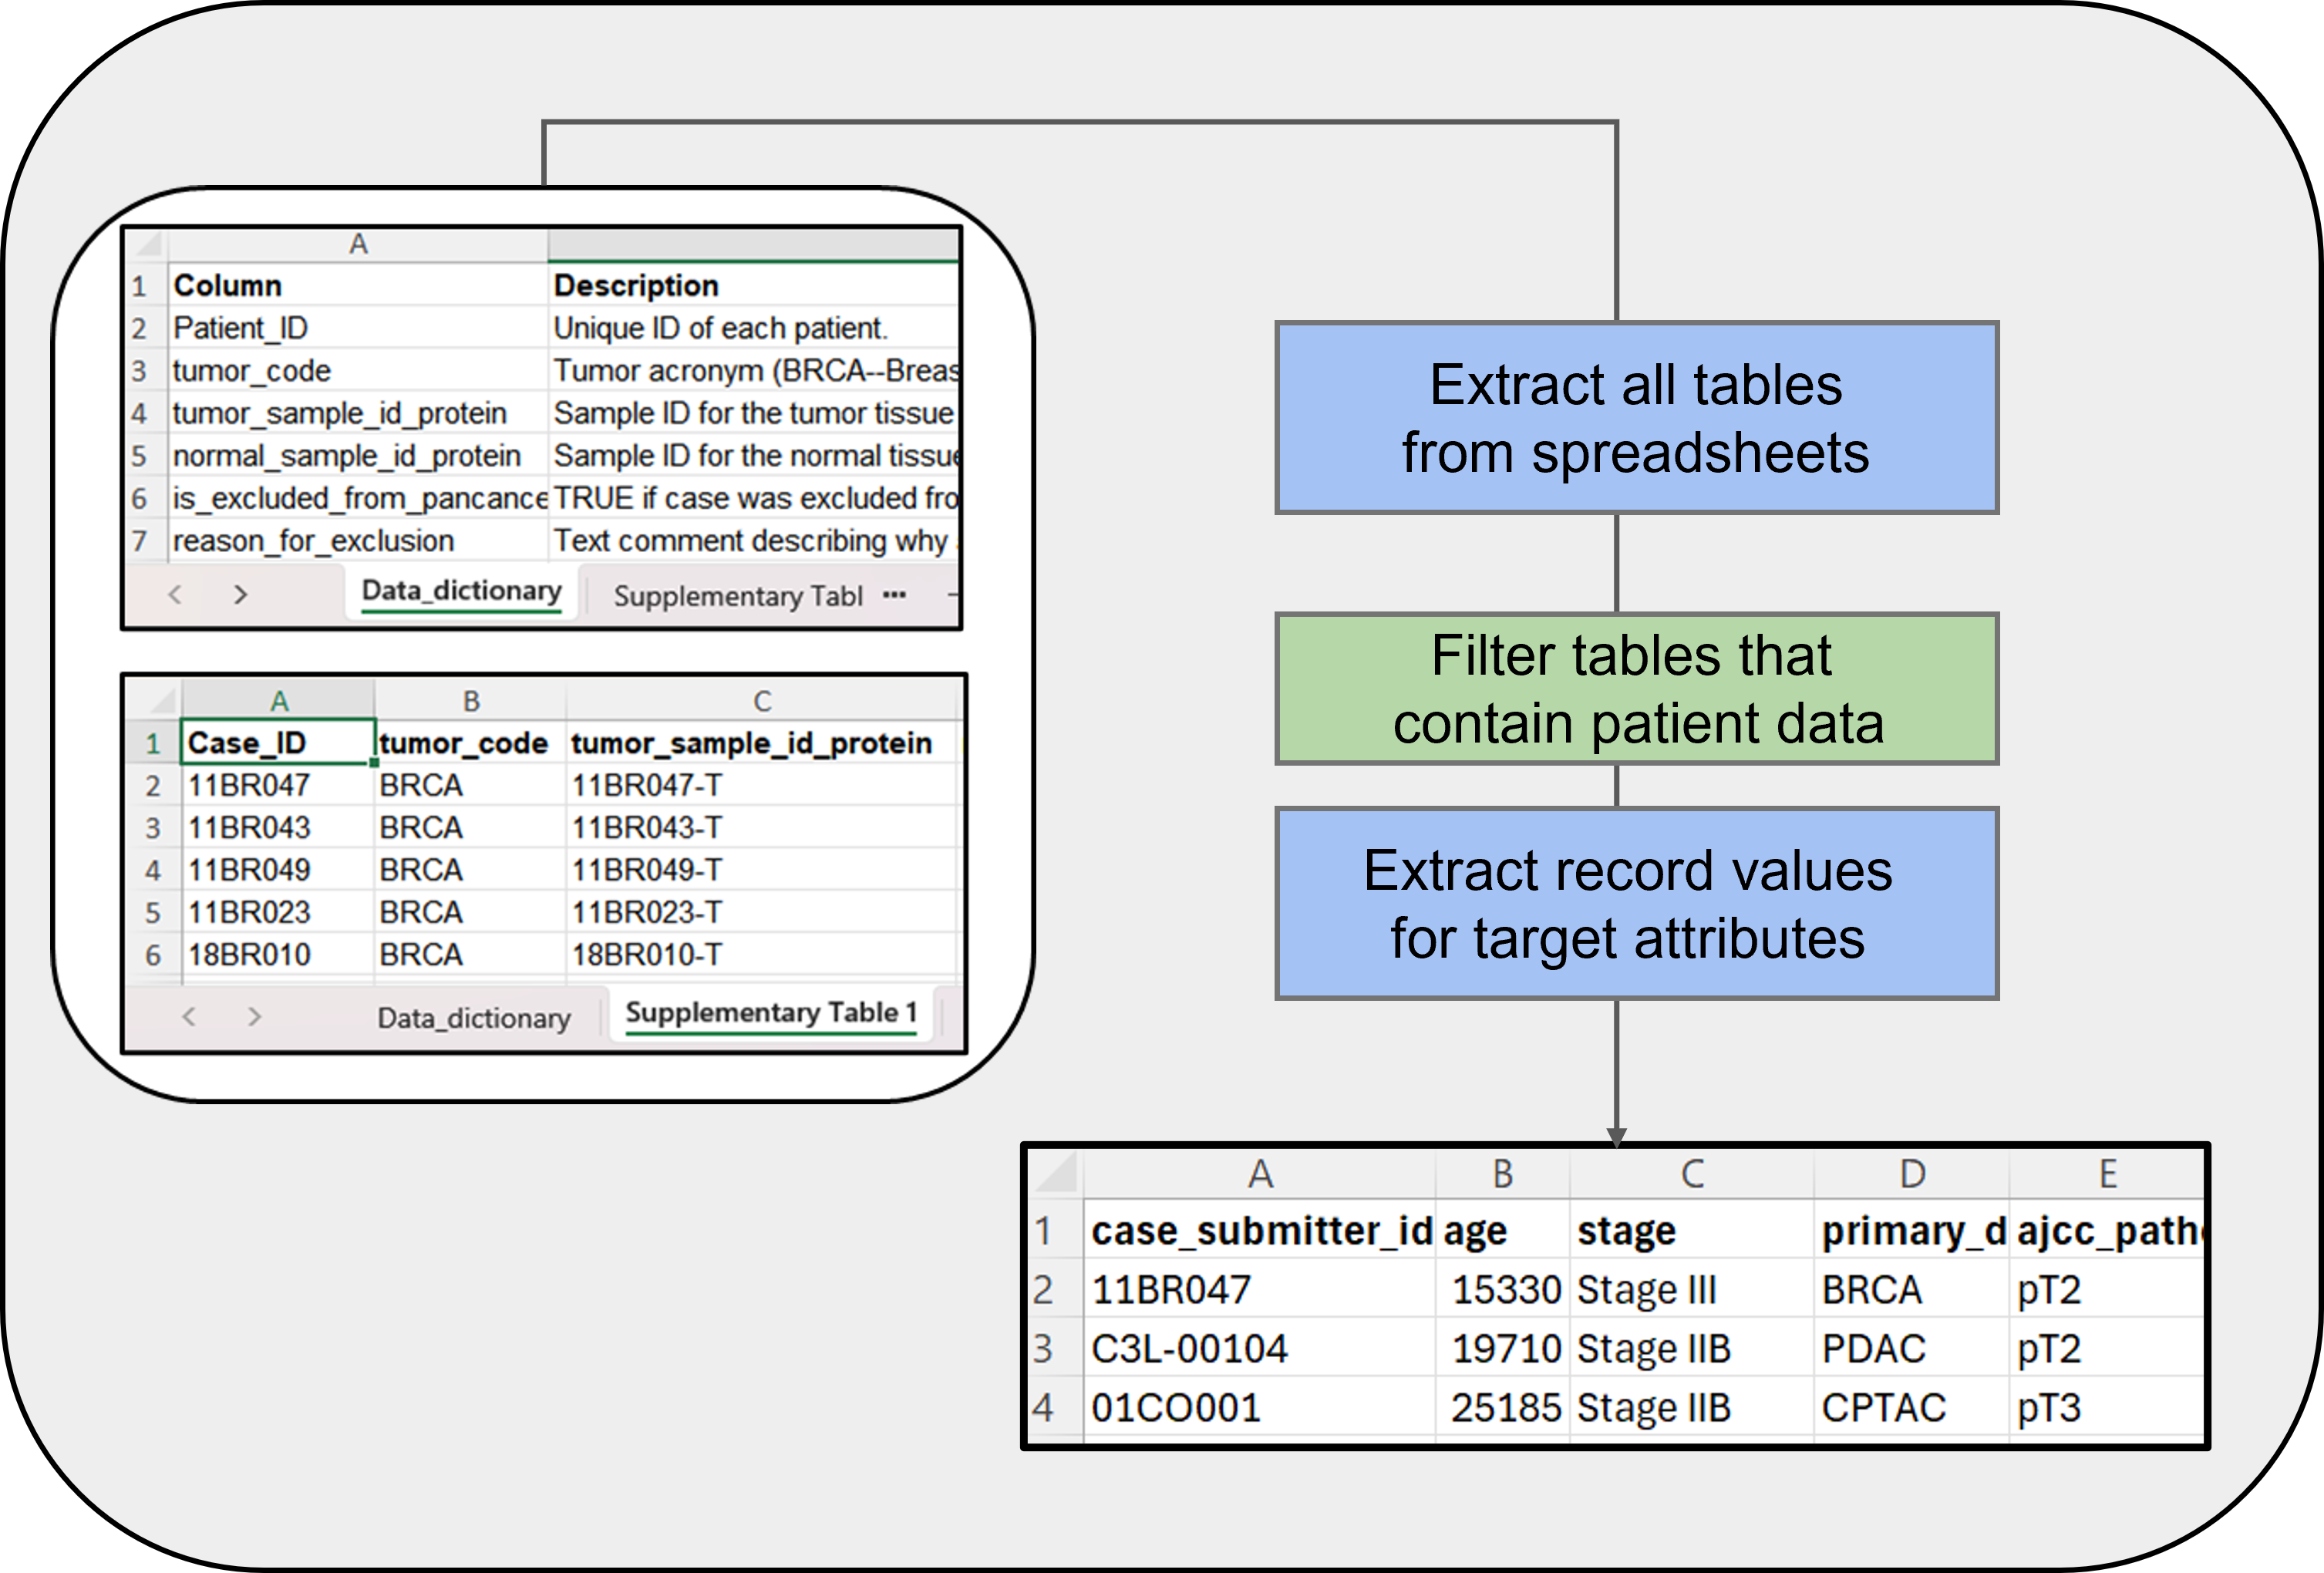
\includegraphics[width=0.48\textwidth]{imgs/biofabric_matching_small.png}
%     \caption{Example of the Medical Schema Matching workload. Three spreadsheets contain several tables and \system{} (1) filters for tables that relate to patient data and (2) matches and extracts the relevant attributes, consolidating a single table with a target schema.}
%     \label{fig:biofabric-matching}
%     % \caption{}
% \end{figure*}

% \begin{itemize}
%     \item {\bf SAPPs:}
%     \begin{itemize}
%         \item {\bf Rental Property Search}
%         \begin{itemize}
%             \item {\bf Dataset:} On the order of 100 to 1k rental property listings in the Boston Metro Area scraped from Zillow
%             \item {\bf Evaluation Task:} Find an apartment that is "modern and attractive with lots of natural sunlight" and within 10 miles of MIT.
%             \item {\bf Evaluation Metric:} For SAPPs I think we want to demonstrate good empirical output quality more than anything else. We may need to create labels by hand for the semantic test (or we can use construction date as a proxy for ``modern"). Limiting our evaluation to precision (as a quality metric) might also make labelling work easier. Alternatively, we can compute Jaccard similarity w/our custom baseline's output.
%             \item {\bf Baseline:} A pipeline built using LangChain with some choice of vision and text model(s).
%         \end{itemize}
%         \item {\bf Legal Discovery}
%         \begin{itemize}
%             \item {\bf Dataset:} 500k enron emails
%             \item {\bf Evaluation Task:} Find emails which (A) are related to fraudulent schemes (i.e., Raptor, Deathstar, Chewco, and/or Fat Boy) and (B) are not quoting from a news article or an article written by someone outside of Enron .
%             \item {\bf Evaluation Metric:} For SAPPs I think we want to demonstrate good empirical output quality more than anything else. We could evaluate PZ against a baseline using Precision@K since we do not have groundtruth labels for this dataset and the dataset is too large to manually label. As an additional evaluation, we could measure recall by using hard-coded logic to label emails (e.g. by checking if each email contains an executives' name and/or fraudulent entities / trading scheme). However, I think this plays second fiddle to the Precision@K evaluation, because we really are hoping to show that the AI system can identify emails which would not be caught by a simple substring match.
%             \item {\bf Baseline:} A pipeline built using LangChain w/some choice of text model(s).
%         \end{itemize}
%     \end{itemize}
%     \item {\bf Document-Driven Discovery}
%     \begin{itemize}
%         \item We can re-use our Enron Emails dataset, but perhaps implement a separate evaluation which is more in-line w/traditional document-driven discovery?
%     \end{itemize}
%     \item {\bf Multimodal Integration}
%     \begin{itemize}
%         \item We can re-use our Rental Property Search dataset, but perhaps implement a separate evaluation which is more in-line w/traditional multimodal integration work?
%     \end{itemize}
    % \item {\bf RAG systems}
    % \begin{itemize}
    %     \item {\bf Internal RAG}
    %     \begin{itemize}
    %         \item {\bf Dataset:} on the order of 20-50 Research Paper PDFs
    %         \item {\bf Evaluation Task:} Extract the title, authors, abstract, and a summary of related work(s) for the given dataset of papers.
    %         \item {\bf Evaluation Metric:} pareto-optimality for runtime vs. cost; measure quality w/accuracy for title, authors, and abstract; can use human evaluation, BLEU scores, and/or GPT-4 for topic summaries.
    %         \item {\bf Baseline:} Langchain pipeline with some state-of-the-art approach to RAG for summarization.
    %     \end{itemize}
    %     \item {\bf External RAG (if we include it in this paper)}
    %     \begin{itemize}
    %         \item {\bf Dataset:} WikiQA (?); we would use (a subset of) the raw Wikipedia dataset and RAG over it
    %         \item {\bf Evaluation Task:} Question answering
    %         \item {\bf Evaluation Metric:} Accuracy of selecting the correct answer sentence
    %         \item {\bf Baseline:} Same state-of-the-art approach to RAG as before, but with multiple datapoints on the runtime/cost vs. quality tradeoff curve for various \#'s of documents retrieved by the vector database. Ideally we can show much better accuracy at fixed runtime and/or cost and vice-versa.
    %     \end{itemize}
    % \end{itemize}
    
%     \item {\bf Schema matching for medical research.}
%     In the medical domain, experimental research in the area of tumor analysis and prevention is often based on large collections of data about patient cases and sample data. 
    
%     The Cancer Research Data Commons (CRDC)~\cite{} provides standardized data formats and metadata dictionaries to foster data exchange and reuse.
%     However, research studies do not always conform to this standard in making data available -- and only sometimes document their data collection and analysis pipelines, often in natural language.
%     Because of this, to reuse previously collected data, new researchers are left with the burden of integrating and standardizing data from different sources.
    
%     We use the real paper from Li et al.~\cite{li2023proteogenomic} as our motivation: in this work, the authors surveyed data from 10 different experimental studies, and manually performed data integration for the different sources.
%     We design a workload to reproduce the steps performed by the original authors of~\cite{li2023proteogenomic} and obtain a single, integrated table that contains patient case metadata (e.g., patient age, tumor stage, ...) for all tumor cases found in the source studies.

%     \textbf{Task description: } 
%     The overall workflow is composed of two sub-tasks: 
%     1) \emph{Filtering:} Each of the original papers from the studies provides supplemental spreadsheets composed of multiple sheets and tables.
%     The goal of this task is to filter all the tables found only to retrieve those that contain the case metadata of interest; 
%     2) \emph{Schema matching:} Given the relevant source tables, identify which of the columns match with the target schema and integrate their content producing a single table compliant with the standard formats provided by the CRDC.

%     \textbf{Evaluation:}
%     For evaluation purposes, we consider 11 spreadsheet files that are provided as datasets in the papers~\cite{Cao_2021, Clark_2019, Dou_2020, Huang_2021, Li_2023, Gillette_2020, Krug_2020, McDermott_2020, Satpathy_2021, Vasaikar_2019,Wang_2021}.
%     Overall, there are 49 individual sheets from which a single table need to be extracted with 15 attributes.
%     We note that not all attributes can be found in the original papers - therefore we consider the correct detection of a missing attribute as part of the ground truth.
%     We synthesize a program with    \system{} that first filters all relevant source tables, and then, extracts the values for the target schema as found in each record of the source tables.
%     Due to the expensiveness of the matching, we sample the first 5 rows for every table.
%     Finally, to evaluate the correctness of the schema matching, for each of the extracted target table attributes, we identify the column from the source containing the extracted values.
%     Suppose no column from the source table contains any of the values for a given target attribute (e.g., due to a model hallucinating or failing to extract any value). In that case, we consider the attribute to be detected as missing.
%     We measure the performance of correctly predicted matches using the micro-average of the F1 score across all target attributes and paper studies.

%     \textbf{Discussion of results}
%     For the {\tt Medical Schema Matching} workload, Figure~\ref{fig:biofabric-results} reports the performance of 9 different synthesized plans that combine two calls to LLMs: one for the filtering step and one for the schema matching step.
%     The most performant, expensive and time-consuming plan is the baseline plan that only resorts to calls to the GPT-4 model.
%     This plan has an F1 score of 56.12\%, but it runs for over 35 minutes.
%     However, thanks to \system{}, we can also generate an alternative plan with the same quality but a much lower runtime: the plan that employs GPT-3.5 for the filtering stage can significantly reduce the processing time, running in around 14 minutes.
    
%     Regarding the total running cost, all plans that employ GPT-4 for the matching stage, which yields the most performance, are significantly pricier than all others - with a maximum cost of 3 USD.
%     However, using \system{}'s capabilities, users can trade off some downstream quality for cost efficiency.
%     Choosing a cheaper plan, such as the one labeled GPT3.5-GEMINI, synthesized using GPT3.5 for the filtering stage and GEMINI   for the matching stage reaches an F1 score of 50\% for a cost of .02 USD. 
 
% \end{itemize}



% \begin{figure*}[t!]
%     \begin{subfigure}[t]{0.48\textwidth}
%         \includegraphics[width=\textwidth]{imgs/enron-eval.png}
%         \caption{Performance of different \system{} plans on the \texttt{Legal Discovery} workload. We highlight the naive plans that use the same model (GPT-4 and Mixtral MoE 7B, respectively) for all operations. \system{} is able to generate plans with up to X runtime savings and Y cost savings at the same quality as the All-GPT4 plan. Similarly, it generates plans with up to X better quality at fixed runtime and cost compared to ALL-MIXTRAL.}
%     \label{fig:enron-result}
%     \end{subfigure}
%     \hfill
%     \begin{subfigure}[t]{0.48\textwidth}
%         \includegraphics[width=\textwidth]{imgs/real-estate-eval-with-bad-plans.png}
%         \caption{Performance of different \system{} plans on the \texttt{Rental Property Search} workload. Based on initial cost estimates, all plans prioritize converting and filtering based on text before processing any image data. \system{} is able to generate plans with up to X runtime savings and Y cost savings compared to plans which do not perform this optimization.}
%     \label{fig:real-estate-result}
%     \end{subfigure}

%     \begin{subfigure}[t]{0.48\textwidth}
%         \includegraphics[width=\textwidth]{imgs/biofabric.png}
%         \caption{Performance of different \system{} plans on the \texttt{Medical Schema Matching} workload.
%         We highlight the ALL-GPT-4 plan that uses GPT-4 for both filtering and matching, and reaches the highest F1 score but at a significant cost. At the same time, PALIMPZEST is able to generate plans that combine different LLMs for the filtering and matching stage, such as GPT-3.5-GPT-4, and GPT3.5-GEMINI (first name corresponding to the model used in filtering).
%         Choosing the GPT3.5-GPT4 plan leads to the same optimal performance with a drastic improvement in runtime, while the GPT-3.5-GEMINI plan sacrifices some performance and runtime for a much lower cost.
%         }
%     \label{fig:biofabric-results}
%     \end{subfigure}
%     % \caption{}
%     \hfill % just placing this here for now, we can definitely move it later (i.e. tomorrow)
%     \begin{subfigure}[t]{0.48\textwidth}
%         \includegraphics[width=\textwidth]{imgs/codegen-easy-eval.png}
%         \caption{Demonstrating the performance improvement(s) of using code generation as an optimization for (some) {\bf convert} operation(s) in \system{} plans. These plans were all run on a variant of the \texttt{Real Estate} workload which used a single convert operation to extract data fields (such as the address, number of bedrooms, etc.), followed by four user-defined filters. As the dataset size increases, the runtime and cost of the plan with a code generated conversion stays roughly constant, while the other \system{} plans' costs increase linearly. \texttt{ALL-GPT} and \texttt{CODEGEN (GPT4)} achieve perfect F1-scores of 1.0 at each point along their respective curves. \texttt{ALL-MIXTRAL} achieves scores in the range [0.8, 1.0].}
%     \label{fig:codegen-results}
%     \end{subfigure}
%     % \caption{}
% \end{figure*}




% \subsection{Micro-benchmarking for Token Reduction}
% \cliu{We can remove this section as quality and cost evaluation have been covered by \autoref{sec:token-reduction}, though the above three scenarios may not show the full benefits. }
% For the sample-based token reduction evaluation, we begin with a training set of 80 VLDB papers to generate an answer heatmap. We then assess the token reduction on a test set comprising 100 VLDB papers. We report comparable results with optimized cost and runtime reduction.

% In our preliminary experiments, we evaluated the questions listed in \autoref{tab:paper_questions}.
% \begin{table}[h]
% \centering
% \caption{Questions about the paper}
% \begin{tabular}{|c|l|}
% \hline
% \textbf{ID} & \textbf{Question}                                  \\ \hline
% Q1           & What is the paper title?           \\ \hline
% Q2           & Who are the authors of the paper?                  \\ \hline
% Q3           & What is the main contribution of the paper?                        \\ \hline
% \end{tabular}
% \label{tab:paper_questions}
% \end{table}


% \noindent \textbf{Comparable Results:}
% We used a binary classifier to compare the test results with the gold answers derived from the context of the full paper. For some questions with lengthy answers, a binary classifier proved insufficient, so we also employed embedding cosine similarity for evaluation.

% We evaluated the output quality with token reduction enabled, as shown in \autoref{fig:qa-acc}. Token reduction works well for simple questions, using less than $5\%$ of the full paper context. However, for more complex questions with lengthy answers, such as Q3 about the paper's contribution, token reduction does not guarantee the accuracy of the results. This is because LLM token generation is highly sensitive to input variations; even a single token change can lead to drastically different outcomes. Although we provide the LLM with input context that includes the ground truth text, it does not guarantee an answer similar to that derived from the entire paper context. The results for Q3 demonstrate that adding more context does not enhance result quality with a token budget exceeding $20\%$, which covers all the ground truth regions. We observed similar results even with cosine similarity evaluation.

% \begin{figure}
%     \centering
%     \includegraphics[width=0.48\textwidth]{imgs/token_reduction/sample/acc/line-questions.pdf}
%     \caption{Question answer binary accuracy over context proportion}
%     \label{fig:qa-acc} 
% \end{figure}


% \noindent \textbf{Runtime and Cost Saving:}
% While delivering comparable results, token reduction demonstrates significant benefits in terms of runtime and cost savings. Profiling the runtime for an LLM vendor is challenging due to network and server load variations. In our evaluation, we profiled the runtime of the LLM using different model serving APIs, including the popular Hugging Face and the well-optimized vLLM, with on-premise hardware. We ran the Mistral-7B-Instruct-v0.2 model on a V100 GPU with 32GB of memory and profiled the query runtime over the test set with varying input tokens.

% \autoref{fig:runtime-vllm} illustrates the query runtime with the vLLM model serving APIs. Since the number of tokens in the answers is relatively consistent, the LLM query runtime increases linearly as the number of input tokens increases. The runtime remains relatively constant when the input context is smaller than $1\%$.
% The Hugging Face evaluation shows similar trends but generally incurs a greater runtime cost due to a lack of optimization.

% In summary, token reduction achieves substantial runtime and cost savings ($80 - 99\%$) without compromising LLM performance.

% % 1*3 figure layout for vllm
% \begin{figure*}
%     \centering
%     \begin{subfigure}[b]{0.3\textwidth}
%         \centering
%         \includegraphics[width=\textwidth]{imgs/token_reduction/sample/runtime/vllm_violin-title.pdf} 
%         \caption{Title}
%         \label{fig:vllm-title}
%     \end{subfigure}
%     \hfill % This adds some horizontal space between the figures
%     \begin{subfigure}[b]{0.3\textwidth}
%         \centering
%         \includegraphics[width=\textwidth]{imgs/token_reduction/sample/runtime/vllm_violin-authors.pdf}
%         \caption{Authors}
%         \label{fig:vllm-auth}
%     \end{subfigure}
%     \hfill % This adds some horizontal space between the figures
%     \begin{subfigure}[b]{0.3\textwidth}
%         \centering
%         \includegraphics[width=\textwidth]{imgs/token_reduction/sample/runtime/vllm_violin-contribution.pdf}
%         \caption{Contribution}
%         \label{fig:vllm-contr}
%     \end{subfigure}
%     \caption{Runtime of the generation with vLLM model serving API}
%     \label{fig:runtime-vllm}
% \end{figure*}

% System performance to evaluate / research questions to answer:
% \begin{itemize}
%     \item Is \texttt{quality} correlated with groundtruth metric(s) for our datasets?
%     \begin{itemize}
%         \item Do we need to use AQP tricks / UDFs to get a sense of quality during sampling?
%     \end{itemize}
%     \item How much does intra-execution re-optimization help our estimation?
%     \item How accurate is our cost model at estimating time and dollars spent?
%     \item What are the throughput(s) we can achieve in this system (for text? images?)
%     \begin{itemize}
%         \item What qualities of the input affect throughput the most?
%     \end{itemize}
% \end{itemize}

